\documentclass{standalone}
\usepackage{tikz}
\usetikzlibrary{patterns, positioning}
\usepackage[sfdefault]{ClearSans} %% option 'sfdefault' activates Clear Sans as the default text font
\usepackage[T1]{fontenc}

\begin{document}
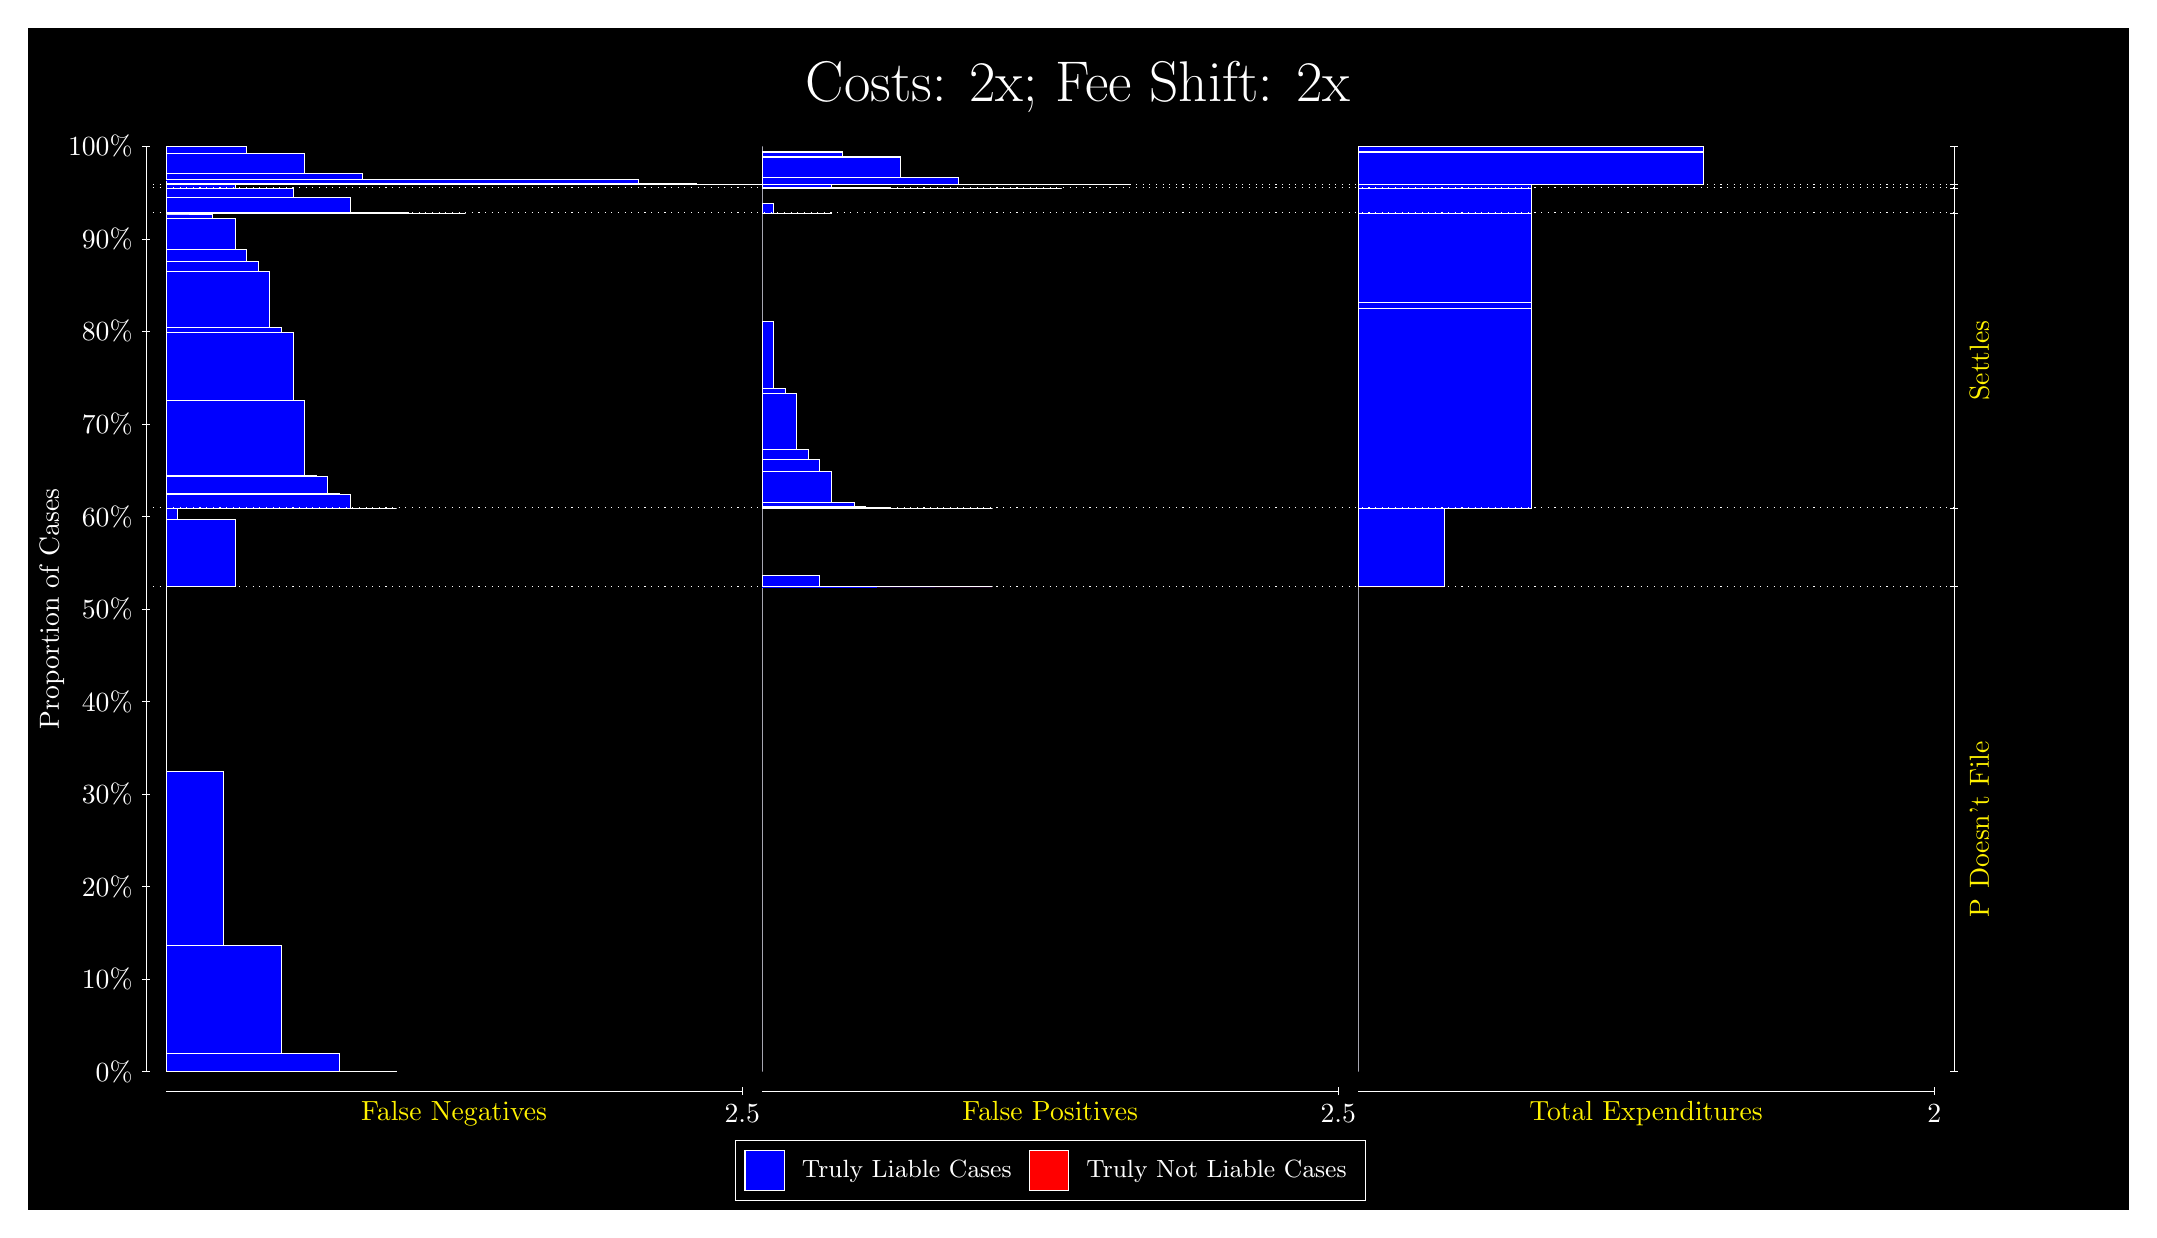
\begin{tikzpicture}
\draw[fill=black] (0,0) rectangle (26.667,15);
\draw[text=white] (0,13.5) rectangle (26.667,15) node[midway] {\huge Costs: 2x; Fee Shift: 2x};
\draw[white, very thin] (1.5,1.75) -- (1.5,13.5);
\node[rotate=90, text=white, anchor=center] at (0.3, 7.625) {Proportion of Cases};
\draw[white, very thin] (1.45,1.75) -- (1.55,1.75);
\node[text=white, anchor=east] at (1.45, 1.75) {0\%};
\draw[white, very thin] (1.45,2.925) -- (1.55,2.925);
\node[text=white, anchor=east] at (1.45, 2.925) {10\%};
\draw[white, very thin] (1.45,4.1) -- (1.55,4.1);
\node[text=white, anchor=east] at (1.45, 4.1) {20\%};
\draw[white, very thin] (1.45,5.275) -- (1.55,5.275);
\node[text=white, anchor=east] at (1.45, 5.275) {30\%};
\draw[white, very thin] (1.45,6.45) -- (1.55,6.45);
\node[text=white, anchor=east] at (1.45, 6.45) {40\%};
\draw[white, very thin] (1.45,7.625) -- (1.55,7.625);
\node[text=white, anchor=east] at (1.45, 7.625) {50\%};
\draw[white, very thin] (1.45,8.8) -- (1.55,8.8);
\node[text=white, anchor=east] at (1.45, 8.8) {60\%};
\draw[white, very thin] (1.45,9.975) -- (1.55,9.975);
\node[text=white, anchor=east] at (1.45, 9.975) {70\%};
\draw[white, very thin] (1.45,11.15) -- (1.55,11.15);
\node[text=white, anchor=east] at (1.45, 11.15) {80\%};
\draw[white, very thin] (1.45,12.325) -- (1.55,12.325);
\node[text=white, anchor=east] at (1.45, 12.325) {90\%};
\draw[white, very thin] (1.45,13.5) -- (1.55,13.5);
\node[text=white, anchor=east] at (1.45, 13.5) {100\%};

\draw[white, very thin] (24.457,1.75) -- (24.457,13.5);
\draw[white, very thin] (24.407,1.75) -- (24.507,1.75);
\node[anchor=west] at (24.407, 1.75) {};
\draw[white, very thin] (24.407,7.9074) -- (24.507,7.9074);
\node[anchor=west] at (24.407, 7.9074) {};
\draw[white, very thin] (24.407,8.908) -- (24.507,8.908);
\node[anchor=west] at (24.407, 8.908) {};
\draw[white, very thin] (24.407,12.654) -- (24.507,12.654);
\node[anchor=west] at (24.407, 12.654) {};
\draw[white, very thin] (24.407,12.973) -- (24.507,12.973);
\node[anchor=west] at (24.407, 12.973) {};
\draw[white, very thin] (24.407,13.02) -- (24.507,13.02);
\node[anchor=west] at (24.407, 13.02) {};
\draw[white, very thin] (24.407,13.5) -- (24.507,13.5);
\node[anchor=west] at (24.407, 13.5) {};

\draw[white, very thin, fill=blue] (1.75,1.75) rectangle (4.6775,1.7523);
\draw[white, very thin, fill=blue] (1.75,1.7523) rectangle (3.9457,1.985);
\draw[white, very thin, fill=blue] (1.75,1.985) rectangle (3.2138,3.3527);
\draw[white, very thin, fill=blue] (1.75,3.3527) rectangle (2.4819,5.5589);
\draw[white, very thin, fill=red] (1.75,5.5589) rectangle (1.75,5.5589);
\draw[white, very thin, fill=blue] (1.75,5.5589) rectangle (1.75,7.9074);
\draw[white, very thin, fill=blue] (1.75,7.9074) rectangle (2.6283,8.7592);
\draw[white, very thin, fill=blue] (1.75,8.7592) rectangle (1.8964,8.9074);
\draw[white, very thin, fill=red] (1.75,8.9074) rectangle (1.75,8.9074);
\draw[white, very thin, fill=blue] (1.75,8.9074) rectangle (1.75,8.908);
\draw[white, very thin, fill=blue] (1.75,8.908) rectangle (4.6775,8.908);
\draw[white, very thin, fill=blue] (1.75,8.908) rectangle (4.3848,8.908);
\draw[white, very thin, fill=blue] (1.75,8.908) rectangle (4.092,9.0842);
\draw[white, very thin, fill=blue] (1.75,9.0842) rectangle (3.9457,9.0876);
\draw[white, very thin, fill=blue] (1.75,9.0876) rectangle (3.7993,9.3073);
\draw[white, very thin, fill=blue] (1.75,9.3073) rectangle (3.6529,9.3283);
\draw[white, very thin, fill=blue] (1.75,9.3283) rectangle (3.5065,10.28);
\draw[white, very thin, fill=blue] (1.75,10.28) rectangle (3.3602,11.137);
\draw[white, very thin, fill=blue] (1.75,11.137) rectangle (3.2138,11.202);
\draw[white, very thin, fill=blue] (1.75,11.202) rectangle (3.0674,11.909);
\draw[white, very thin, fill=blue] (1.75,11.909) rectangle (2.921,12.036);
\draw[white, very thin, fill=blue] (1.75,12.036) rectangle (2.7746,12.192);
\draw[white, very thin, fill=blue] (1.75,12.192) rectangle (2.6283,12.581);
\draw[white, very thin, fill=blue] (1.75,12.581) rectangle (2.4819,12.585);
\draw[white, very thin, fill=blue] (1.75,12.585) rectangle (2.3355,12.639);
\draw[white, very thin, fill=blue] (1.75,12.639) rectangle (2.1891,12.645);
\draw[white, very thin, fill=blue] (1.75,12.645) rectangle (2.0428,12.645);
\draw[white, very thin, fill=blue] (1.75,12.645) rectangle (1.8964,12.654);
\draw[white, very thin, fill=red] (1.75,12.654) rectangle (1.75,12.654);
\draw[white, very thin, fill=blue] (1.75,12.654) rectangle (1.75,12.654);
\draw[white, very thin, fill=blue] (1.75,12.654) rectangle (5.5558,12.654);
\draw[white, very thin, fill=blue] (1.75,12.654) rectangle (4.8239,12.659);
\draw[white, very thin, fill=blue] (1.75,12.659) rectangle (4.092,12.848);
\draw[white, very thin, fill=blue] (1.75,12.848) rectangle (3.3602,12.971);
\draw[white, very thin, fill=blue] (1.75,12.971) rectangle (2.6283,12.973);
\draw[white, very thin, fill=red] (1.75,12.973) rectangle (1.75,12.973);
\draw[white, very thin, fill=blue] (1.75,12.973) rectangle (2.6283,13.018);
\draw[white, very thin, fill=blue] (1.75,13.018) rectangle (1.8964,13.02);
\draw[white, very thin, fill=red] (1.75,13.02) rectangle (1.75,13.02);
\draw[white, very thin, fill=blue] (1.75,13.02) rectangle (1.75,13.02);
\draw[white, very thin, fill=blue] (1.75,13.02) rectangle (9.9471,13.02);
\draw[white, very thin, fill=blue] (1.75,13.02) rectangle (9.2152,13.02);
\draw[white, very thin, fill=blue] (1.75,13.02) rectangle (8.4834,13.031);
\draw[white, very thin, fill=blue] (1.75,13.031) rectangle (7.7515,13.076);
\draw[white, very thin, fill=blue] (1.75,13.076) rectangle (7.0196,13.077);
\draw[white, very thin, fill=blue] (1.75,13.077) rectangle (6.2877,13.077);
\draw[white, very thin, fill=blue] (1.75,13.077) rectangle (5.7022,13.077);
\draw[white, very thin, fill=blue] (1.75,13.077) rectangle (5.5558,13.077);
\draw[white, very thin, fill=blue] (1.75,13.077) rectangle (4.9703,13.077);
\draw[white, very thin, fill=blue] (1.75,13.077) rectangle (4.2384,13.152);
\draw[white, very thin, fill=blue] (1.75,13.152) rectangle (3.5065,13.408);
\draw[white, very thin, fill=blue] (1.75,13.408) rectangle (2.7746,13.496);
\draw[white, very thin, fill=blue] (1.75,13.496) rectangle (2.0428,13.5);
\draw[white, very thin, fill=red] (1.75,13.5) rectangle (1.75,13.5);
\draw[white, very thin, fill=blue] (1.75,13.5) rectangle (1.75,13.5);
\draw[white, very thin, fill=red] (9.3189,1.75) rectangle (9.3189,1.75);
\draw[white, very thin, fill=blue] (9.3189,1.75) rectangle (9.3189,7.9074);
\draw[white, very thin, fill=red] (9.3189,7.9074) rectangle (12.246,7.9074);
\draw[white, very thin, fill=blue] (9.3189,7.9074) rectangle (12.246,7.9074);
\draw[white, very thin, fill=blue] (9.3189,7.9074) rectangle (11.515,7.9074);
\draw[white, very thin, fill=blue] (9.3189,7.9074) rectangle (10.783,7.908);
\draw[white, very thin, fill=blue] (9.3189,7.908) rectangle (10.051,8.0562);
\draw[white, very thin, fill=blue] (9.3189,8.0562) rectangle (9.3189,8.908);
\draw[white, very thin, fill=red] (9.3189,8.908) rectangle (12.246,8.908);
\draw[white, very thin, fill=blue] (9.3189,8.908) rectangle (12.246,8.908);
\draw[white, very thin, fill=red] (9.3189,8.908) rectangle (11.954,8.908);
\draw[white, very thin, fill=blue] (9.3189,8.908) rectangle (11.954,8.908);
\draw[white, very thin, fill=red] (9.3189,8.908) rectangle (11.661,8.908);
\draw[white, very thin, fill=blue] (9.3189,8.908) rectangle (11.661,8.908);
\draw[white, very thin, fill=blue] (9.3189,8.908) rectangle (11.515,8.908);
\draw[white, very thin, fill=red] (9.3189,8.908) rectangle (11.368,8.908);
\draw[white, very thin, fill=blue] (9.3189,8.908) rectangle (11.368,8.908);
\draw[white, very thin, fill=blue] (9.3189,8.908) rectangle (11.222,8.908);
\draw[white, very thin, fill=red] (9.3189,8.908) rectangle (11.075,8.908);
\draw[white, very thin, fill=blue] (9.3189,8.908) rectangle (11.075,8.908);
\draw[white, very thin, fill=blue] (9.3189,8.908) rectangle (10.929,8.9162);
\draw[white, very thin, fill=blue] (9.3189,8.9162) rectangle (10.783,8.9165);
\draw[white, very thin, fill=blue] (9.3189,8.9165) rectangle (10.636,8.9225);
\draw[white, very thin, fill=blue] (9.3189,8.9225) rectangle (10.49,8.977);
\draw[white, very thin, fill=blue] (9.3189,8.977) rectangle (10.344,8.9806);
\draw[white, very thin, fill=blue] (9.3189,8.9806) rectangle (10.197,9.3702);
\draw[white, very thin, fill=blue] (9.3189,9.3702) rectangle (10.051,9.5259);
\draw[white, very thin, fill=blue] (9.3189,9.5259) rectangle (9.9044,9.653);
\draw[white, very thin, fill=blue] (9.3189,9.653) rectangle (9.758,10.359);
\draw[white, very thin, fill=blue] (9.3189,10.359) rectangle (9.6116,10.424);
\draw[white, very thin, fill=blue] (9.3189,10.424) rectangle (9.4652,11.282);
\draw[white, very thin, fill=blue] (9.3189,11.282) rectangle (9.3189,12.654);
\draw[white, very thin, fill=red] (9.3189,12.654) rectangle (10.197,12.654);
\draw[white, very thin, fill=blue] (9.3189,12.654) rectangle (10.197,12.655);
\draw[white, very thin, fill=blue] (9.3189,12.655) rectangle (9.4652,12.778);
\draw[white, very thin, fill=blue] (9.3189,12.778) rectangle (9.3189,12.973);
\draw[white, very thin, fill=red] (9.3189,12.973) rectangle (13.125,12.973);
\draw[white, very thin, fill=blue] (9.3189,12.973) rectangle (13.125,12.973);
\draw[white, very thin, fill=blue] (9.3189,12.973) rectangle (12.393,12.973);
\draw[white, very thin, fill=blue] (9.3189,12.973) rectangle (11.661,12.973);
\draw[white, very thin, fill=blue] (9.3189,12.973) rectangle (10.929,12.974);
\draw[white, very thin, fill=blue] (9.3189,12.974) rectangle (10.197,13.02);
\draw[white, very thin, fill=red] (9.3189,13.02) rectangle (14.003,13.02);
\draw[white, very thin, fill=blue] (9.3189,13.02) rectangle (14.003,13.02);
\draw[white, very thin, fill=red] (9.3189,13.02) rectangle (13.271,13.02);
\draw[white, very thin, fill=blue] (9.3189,13.02) rectangle (13.271,13.02);
\draw[white, very thin, fill=red] (9.3189,13.02) rectangle (12.539,13.02);
\draw[white, very thin, fill=blue] (9.3189,13.02) rectangle (12.539,13.024);
\draw[white, very thin, fill=blue] (9.3189,13.024) rectangle (11.807,13.112);
\draw[white, very thin, fill=red] (9.3189,13.112) rectangle (11.807,13.112);
\draw[white, very thin, fill=blue] (9.3189,13.112) rectangle (11.807,13.112);
\draw[white, very thin, fill=blue] (9.3189,13.112) rectangle (11.075,13.367);
\draw[white, very thin, fill=blue] (9.3189,13.367) rectangle (11.075,13.368);
\draw[white, very thin, fill=blue] (9.3189,13.368) rectangle (10.344,13.428);
\draw[white, very thin, fill=blue] (9.3189,13.428) rectangle (10.344,13.443);
\draw[white, very thin, fill=blue] (9.3189,13.443) rectangle (9.6116,13.443);
\draw[white, very thin, fill=blue] (9.3189,13.443) rectangle (9.6116,13.443);
\draw[white, very thin, fill=red] (9.3189,13.443) rectangle (9.3189,13.443);
\draw[white, very thin, fill=blue] (9.3189,13.443) rectangle (9.3189,13.5);
\draw[white, very thin, fill=red] (16.888,1.75) rectangle (16.888,1.75);
\draw[white, very thin, fill=blue] (16.888,1.75) rectangle (16.888,7.9074);
\draw[white, very thin, fill=red] (16.888,7.9074) rectangle (17.986,7.9074);
\draw[white, very thin, fill=blue] (16.888,7.9074) rectangle (17.986,8.908);
\draw[white, very thin, fill=red] (16.888,8.908) rectangle (19.083,8.908);
\draw[white, very thin, fill=blue] (16.888,8.908) rectangle (19.083,11.447);
\draw[white, very thin, fill=red] (16.888,11.447) rectangle (19.083,11.447);
\draw[white, very thin, fill=blue] (16.888,11.447) rectangle (19.083,11.519);
\draw[white, very thin, fill=red] (16.888,11.519) rectangle (19.083,11.519);
\draw[white, very thin, fill=blue] (16.888,11.519) rectangle (19.083,12.654);
\draw[white, very thin, fill=red] (16.888,12.654) rectangle (19.083,12.654);
\draw[white, very thin, fill=blue] (16.888,12.654) rectangle (19.083,12.973);
\draw[white, very thin, fill=red] (16.888,12.973) rectangle (19.083,12.973);
\draw[white, very thin, fill=blue] (16.888,12.973) rectangle (19.083,13.02);
\draw[white, very thin, fill=red] (16.888,13.02) rectangle (21.279,13.02);
\draw[white, very thin, fill=blue] (16.888,13.02) rectangle (21.279,13.427);
\draw[white, very thin, fill=red] (16.888,13.427) rectangle (21.279,13.427);
\draw[white, very thin, fill=blue] (16.888,13.427) rectangle (21.279,13.443);
\draw[white, very thin, fill=red] (16.888,13.443) rectangle (21.279,13.443);
\draw[white, very thin, fill=blue] (16.888,13.443) rectangle (21.279,13.5);
\draw[white, dotted] (1.5,7.9074) -- (24.457,7.9074);
\draw[white, dotted] (1.5,8.908) -- (24.457,8.908);
\draw[white, dotted] (1.5,12.654) -- (24.457,12.654);
\draw[white, dotted] (1.5,12.973) -- (24.457,12.973);
\draw[white, dotted] (1.5,13.02) -- (24.457,13.02);
\draw[white, very thin] (1.75,1.5) -- (9.0689,1.5);
\node[text=yellow, anchor=north] at (5.4094, 1.5) {False Negatives};
\draw[white, very thin] (9.0689,1.45) -- (9.0689,1.55);
\node[text=white, anchor=north] at (9.0689, 1.45) {2.5};

\draw[white, very thin] (9.3189,1.5) -- (16.638,1.5);
\node[text=yellow, anchor=north] at (12.978, 1.5) {False Positives};
\draw[white, very thin] (16.638,1.45) -- (16.638,1.55);
\node[text=white, anchor=north] at (16.638, 1.45) {2.5};

\draw[white, very thin] (16.888,1.5) -- (24.207,1.5);
\node[text=yellow, anchor=north] at (20.547, 1.5) {Total Expenditures};
\draw[white, very thin] (24.207,1.45) -- (24.207,1.55);
\node[text=white, anchor=north] at (24.207, 1.45) {2};

\node[text=yellow, centered, rotate=90] at (24.777, 4.8287) {P Doesn't File};

\node[text=yellow, centered, rotate=90] at (24.777, 10.781) {Settles};




\draw (12.978300999999998,1.5) node[draw=none] (baseCoordinate) {};
\begin{scope}[align=center]
        \matrix[scale=0.5, draw=white, below=0.5cm of baseCoordinate, nodes={draw}, column sep=0.1cm]{
            \node[rectangle, draw, minimum width=0.5cm, minimum height=0.5cm, fill=blue] {}; &
            \node[draw=none, font=\small, text=white] (B) {Truly Liable Cases}; &
            \node[rectangle, draw, minimum width=0.5cm, minimum height=0.5cm, fill=red] {}; &
            \node[draw=none, font=\small, text=white] (B) {Truly Not Liable Cases}; \\
            };
\end{scope}

\end{tikzpicture}
\end{document}